\begin{figure*}[p]
\centering
\begin{subfigure}[t]{\columnwidth}
  \centering
  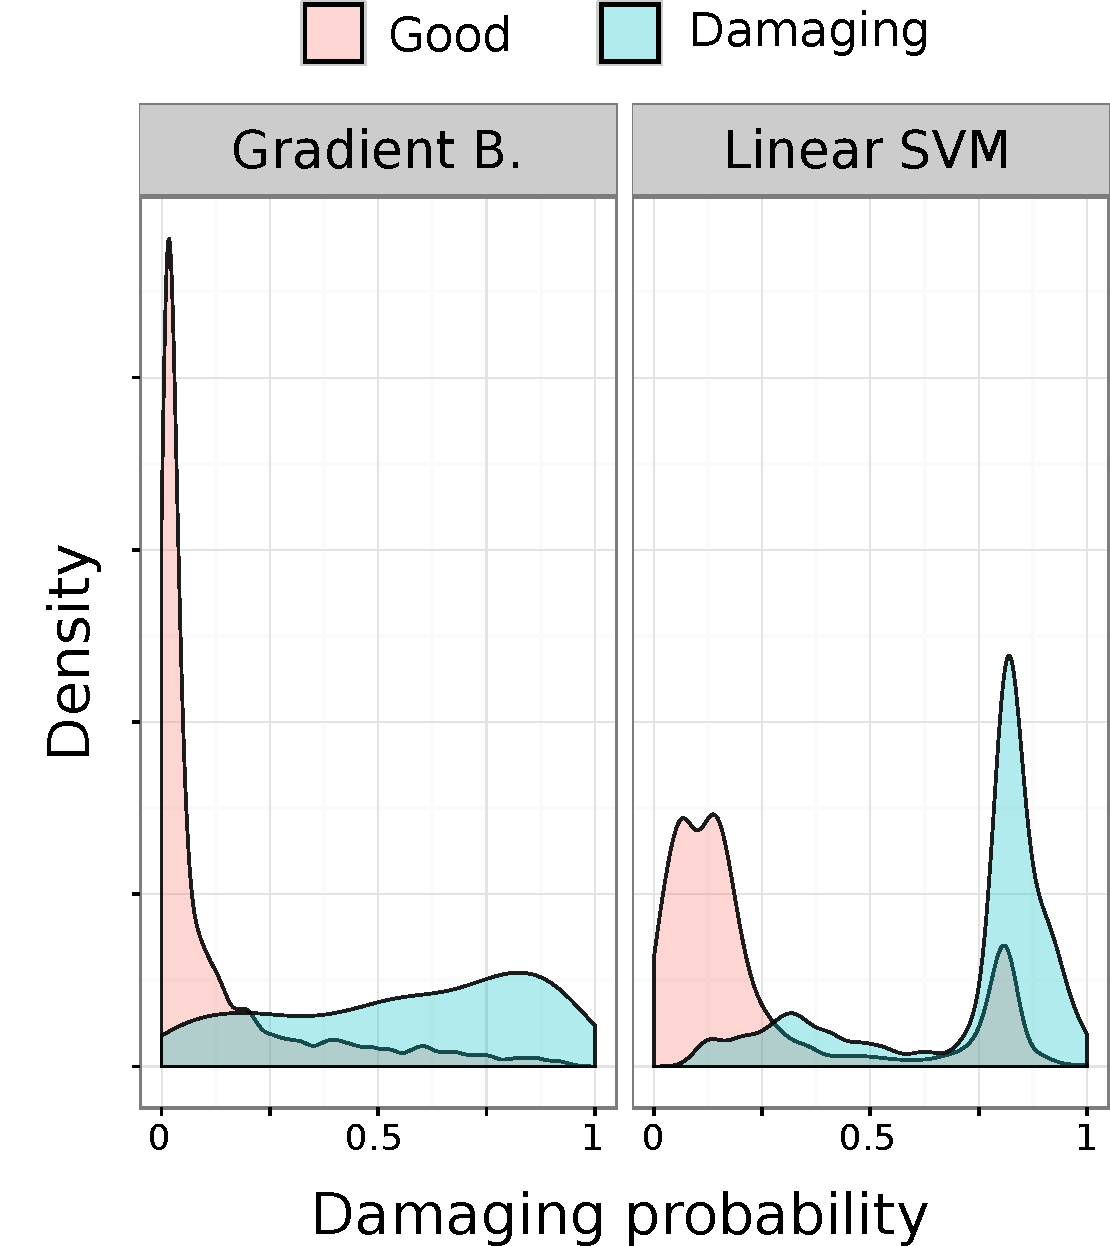
\includegraphics[width=.3\textwidth]{figures/natural_damaging_gb_vs_svc}
  \caption{No injected features}
  \label{fig:natural_damaging_gb_bs_svc}
\end{subfigure}~~
\begin{subfigure}[t]{\columnwidth}
  \centering
  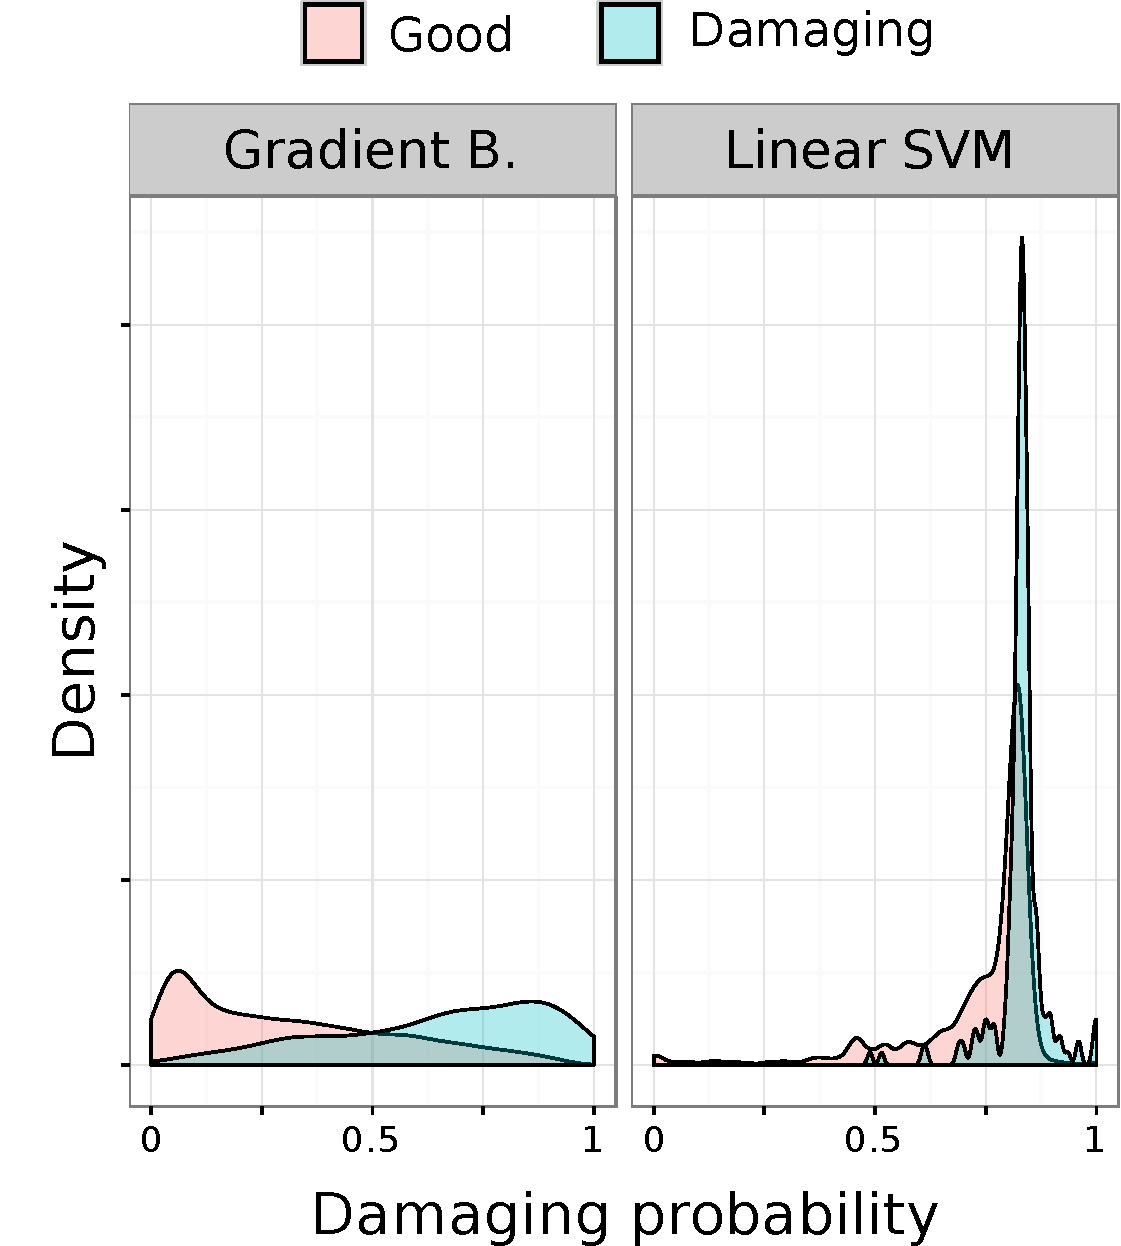
\includegraphics[width=.3\textwidth]{figures/anon_damaging_gb_vs_svc}
  \caption{Everyone is anonymous}
  \label{fig:anon_damaging_gb_bs_svc}
\end{subfigure}~~
\begin{subfigure}[t]{\columnwidth}
  \centering
  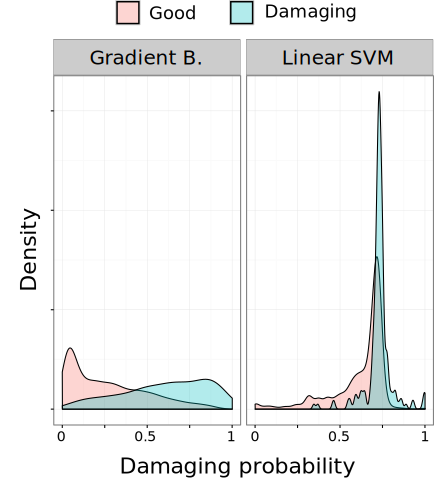
\includegraphics[width=.3\textwidth]{figures/newcomer_damaging_gb_vs_svc}
  \caption{Everyone is newly registered}
  \label{fig:newcomer_damaging_gb_bs_svc}
\end{subfigure}
\caption{The distributions of the probability of a single edit being scored as ``damaging'' based on injected features for the target user-class is presented.  Note that when injecting user-class features (anon, newcomer), all other features are held constant.}
\label{fig:prediction_error_for_anons_and_newcomers}
\end{figure*}
